% C.17 30-60-90, ∠C=90, ∠A=30, AB=10
\documentclass[tikz,border=4pt]{standalone}
\usepackage{ctex}
\usepackage{amsmath}
\usetikzlibrary{calc, arrows.meta}
\begin{document}
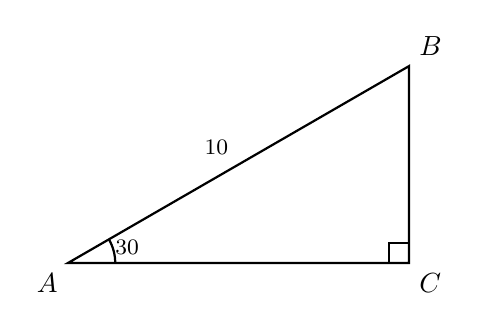
\begin{tikzpicture}[scale=0.5, thick]
  % AC along x-axis, C at right angle; AB hypotenuse=10, ∠A=30
  % AC = 10 cos30 = 5√3 ≈ 8.66, BC = 10 sin30 = 5
  \coordinate (A) at (0,0);
  \coordinate (C) at ({5*sqrt(3)},0);
  \coordinate (B) at ({5*sqrt(3)},5);
  \draw (A) -- (C) -- (B) -- cycle;
  \draw ({5*sqrt(3)-0.5},0) -- ({5*sqrt(3)-0.5},0.5) -- ({5*sqrt(3)},0.5);
  \node[below left] at (A) {$A$};
  \node[below right] at (C) {$C$};
  \node[above right] at (B) {$B$};
  \draw (1.2,0) arc (0:30:1.2);
  \node[font=\footnotesize] at (1.5,0.4) {$30°$};
  \node[font=\footnotesize, above left] at ($(A)!0.5!(B)$) {$10$};
\end{tikzpicture}
\end{document}
